% !TeX root = RJwrapper.tex
\title{\pkg{robslopes}: Efficient Computation of the (Repeated) Median Slope}
\author{by Jakob Raymaekers}

\maketitle

\abstract{
Modern use of slope estimation often involves the (repeated) estimation of a large number of slopes on a large number of data points. Some of the most popular non-parametric and robust alternatives to the least squares estimator are the Theil-Sen and Siegel's repeated median slope estimators. The \CRANpkg{robslopes} package contains fast algorithms for these slope estimators. The implemented randomized algorithms run in $\mathcal{O}(n\log(n))$ and $\mathcal{O}(n\log^2(n))$ expected time respectively and use $\mathcal{O}(n)$ space. They achieve speedups up to a factor $10^3$ compared with existing implementations for common sample sizes, as illustrated in a benchmark study, and they allow for the possibility of estimating the slopes on samples of size $10^5$ and larger thanks to the limited space usage. Finally, the original algorithms are adjusted in order to properly handle duplicate values in the data set.
}

\section{Introduction}

The Theil-Sen estimator \citep{Theil1950, sen1968estimates} is arguably the most popular non-parametric and robust alternative to the least squares estimator for estimating the slope in simple linear regression. A variation on this estimator, Siegel's repeated median slope \citep{siegel1982robust}, was the first slope estimator to attain the maximal breakdown value of 50 \%, which roughly means that it can withstand up to 50\% of outliers in the data. Since their introduction, these estimators have seen widespread use in a variety of applications including signal extraction \citep{davies2004robust, gather2006online}, filtering  \citep{fried2006repeated, bernholt2006modified, fried2007weighted, gelper2010robust}, computer vision \cite{meer1991robust}, climatology \citep{zhang2000temperature, zhai2005trends, kosaka2013recent} and very recently differentially private estimation \citep{alabi2020differentially,fu2021attackresistant}.\par
Several implementations of these estimators exist, most notably in the R packages \CRANpkg{deming} \citep{R:deming}, \CRANpkg{zyp} \citep{R:zyp}, \CRANpkg{mblm} \citep{R:mblm}, and \CRANpkg{RobustLinearReg} \citep{R:RobustLinearReg}, all publicly available on CRAN. Despite their popularity and importance, all of these publicly available implementations are based on a brute-force computation of the (repeated) median slope. Given a sample of $n$ observations, this approach requires a computational cost of $\mathcal{O}(n^2)$ as well as $\mathcal{O}(n^2)$ space. This makes the currently available implementations unsuitable for modern applications involving larger data sets as they are rather slow and potentially use prohibitively large amounts of storage space.\par
Nevertheless, there exist several algorithms for the Theil-Sen and repeated median estimators which run in quasilinear time and require only $\mathcal{O}(n)$ space. For the Theil-Sen estimator, \citet{cole1989optimal}, \citet{katz1993optimal}, and \citet{bronnimann1998optimal} proposed algorithms running in $\mathcal{O}(n\log(n))$ deterministic time. A randomized algorithm requiring $\mathcal{O}(n\log(n))$-expected time was proposed in \citet{matouvsek1991randomized}, \citet{dillencourt1992randomized} and \citet{Shafer1993RandomizingOG}. For the repeated median slope, \citet{stein1992finding}, \citet{matouvsek1993efficient} and \citet{matouvsek1998efficient} proposed algorithms running in $\mathcal{O}(n\log(n))$ and $\mathcal{O}(n\log(n)^2)$ (-expected) time. A potential explanation for these algorithms not being available in R may be twofold. Firstly, they are all more involved than brute-force computation of the median slopes and sample implementations in other programming languages are scarce, if available at all. Secondly, most of them make efficient use of features not (readily) available in R, such as pointers and in-place assignment, as well as complex data structures.\par
In this article we discuss the R package \CRANpkg{robslopes} \citep{R:robslopes} which contains implementations of the randomized algorithms by \citet{matouvsek1991randomized} and \citet{matouvsek1998efficient} for the Theil-Sen and repeated median estimators respectively. The original algorithms have been adjusted in order to properly deal with potential duplicates in the data. We start by briefly reviewing the problem setting and the estimators. Next, we present a rough outline of the key ideas underlying the algorithms and a brief description of the usage of the functions in the package. We end with a benchmarking study comparing the implementation with existing implementations in publicly available R packages and concluding remarks.


\section{The Theil-Sen and repeated median estimators}\label{sec:meth}

The typical problem setting of slope estimation is that of the simple linear model. Suppose we have $n$ observations $(x_i, y_i)$ which follow the model
\begin{equation*}
y_i = \alpha + \beta x_i + e_i
\end{equation*}
where $\alpha$ and $\beta$ are the (unknown) true intercept and slope parameters and $e_i$ represents the noise. The most popular estimator for the regression coefficients is the ordinary least squares (OLS) estimator, i.e. the $(\alphah, \betah)$ minimizing $\sum_{i=1}^{n}{(y_i - \alphah-\betah x_i)^2}$. The OLS estimator possesses several attractive properties, including ease of computation and interpretation and optimal performance when the errors are i.i.d. and follow a normal distribution. Despite these properties, it is well known that the OLS estimator is very sensitive to outliers and can have a quickly deteriorating performance as the error term deviates from normality. For these reasons, many alternatives have been suggested, of which the Theil-Sen estimator and Siegel's repeated median slope are two popular and intuitively attractive examples.\par
The Theil-Sen (TS) estimator \citep{Theil1950, sen1968estimates} of $\beta$ is defined as the median of the slopes of all the lines determined by two different observations $(x_i,y_i)$ and $(x_j, y_j)$:
\begin{equation*}
\betahTS(\bx,\by)=\med_{i\neq j} \frac{y_i - y_j}{x_i - x_j},
\end{equation*}
where the median avoids $i=j$ as the slope through one point is undefined and where $\bx = x_1, \ldots, x_n$ and $\by = y_1, \ldots, y_n$. In case there are duplicate values in $x_1,\ldots,x_n$, the proposal of \cite{sen1968estimates} is to only include the slopes which are constructed using two observations with different $x$-values and we adopt this approach here.\par
The TS estimator has been analyzed extensively from a theoretical point of view. \cite{sen1968estimates} showed its asymptotic normality and equivariance properties. In particular, we have
\begin{enumerate}
\item scale equivariance: $\betahTS(\bx,c\by ) = c\betahTS(\bx,\by) $ for all $c \in \mathbb{R}$
\item regression equivariance $\betahTS(\bx,\by + a\bx) = \betahTS(\bx,\by)  + a$ for all $a \in \mathbb{R}$,
\end{enumerate}
but the estimator is not equivariant under affine transformations of both predictor and response variables. \cite{Wang2005} give precise conditions for the unbiasedness of the TS estimator and \citep{wilcox1998note} studied its behavior in the case of heteroscedastic errors. From a robust statistics perspective, it is known that the TS estimator is much more robust against outliers than the OLS estimator (see \cite{rousseeuw2005robust}). In particular, it has a bounded influence function \citep{Hampel:IFapproach} and its breakdown value is $1 - \sqrt{\frac{1}{2}} \approx 0.293 \%$, where the latter can be roughly interpreted as the maximum percentage of contaminated samples that the estimator can handle (see \cite{Donoho:BDP} for an exact definition). Finally, its maximum bias properties under contamination have been studied by \cite{adrover2004bias}.\\

The search for a slope estimator with a breakdown value higher than 30\% prompted Siegel to propose the repeated median (RM) slope \citep{siegel1982robust}. It is the first slope estimator attaining the maximal breakdown value of 50\%. The repeated median estimator of $\beta$ is computed by first calculating the median slope per observation $x_i$, yielding $n$ values, and then taking the median of these values:
\begin{equation*}
\betahRM(\bx,\by)=\med_i \med_{j\neq i} \frac{y_j - y_i}{x_j - x_i},
\end{equation*}
where now the inner median avoids $i=j$. We handle duplicate values in $x_1,\ldots,x_n$ by skipping them in the computation of the inner median, in the same spirit as duplicate handling for the TS estimator. The consistency, unbiasedness and efficiency of the RM estimator were discussed by \cite{siegel1982robust}, whereas the asymptotic normality was analyzed in \cite{hossjer1994asymptotics}. The estimator was designed to have a 50 \% asymptotic breakdown value, and like the TS estimator, its influence function is also bounded \citep{rousseeuw1992new, rousseeuw1995sensitivity, rousseeuw2005robust}. Finally, it possesses the same equivariance properties as the TS estimator, i.e. it is both scale and regression equivariant but not affine equivariant, and its maximum bias properties are also discussed in \cite{adrover2004bias}.\par

It is clear that both $\betahTS$ and $\betahRM$ can be computed by calculating all $\frac{n(n-1)}{2}$ pairwise slopes, and selecting the median or repeated median of these slopes. Clearly, this brute-force approach has a $\mathcal{O}(n^2)$ computational cost, and the available implementations of this approach also require storing the $\mathcal{O}(n^2)$ slopes. In the next section, we describe the more efficient algorithms implemented in the \pkg{robslopes} package.



While not the main focus of this article, it is worth mentioning that the intercept can be estimated in several ways. We opt for the most straight-forward approach of taking the median of the residuals as the estimator for $\alpha$:
\begin{equation*}
\alphah = \med_i \left(y_i - \betah x_i\right),
\end{equation*}
where $\betah$ can be $\betahTS$ or $\betahRM$.\par

\section{Randomized algorithms for slope selection}\label{sec:algo}
The R-package \pkg{robslopes} contains an implementation of the randomized algorithm by \citet{matouvsek1991randomized} for the Theil-Sen estimator and 
the algorithm of \citet{matouvsek1993efficient, matouvsek1998efficient} for the repeated median estimator. Unlike in their original proposals, we haven taken into account the case of possible duplicate values in the $x_i$ and adjusted the algorithms to work properly in that case as well. We now briefly outline these algorithms without going too much into detail. For specific details and a complete description we refer to the original references and our code.\par
Suppose we are given $n$ data points $(x_i, y_i)$ with $i = 1,\ldots,n$ and we are interested in the median (or more generally, any order statistic) of the slopes formed by connecting two data points. The main idea behind the algorithms is to consider each observed data point $(x_i, y_i)$ in dual space by associating it with the line 
$$v = x_i u - y_i.$$
We will denote the coordinates in dual space with $(u,v)$ in the following. It can be verified that the $u$-coordinate of the intersection of two lines in dual space (also called ``intersection abscissa'' (IA)) is equal to the slope of the line passing through the two points in the original space. Therefore, the problem of finding order statistics of slopes can be translated into the problem of finding order statistics of intersection abscissas in dual space. To find these order statistics in dual space, the algorithms use the following idea. Given an interval $(\ul,\uh]$ in dual space, the number of IAs in that interval can be computed by counting the number of inversions in a certain permutation. For a permutation $\pi$ on $1,\ldots,n$, an inversion is a pair of elements $(\pi(i),\pi(j))$ for which $i<j$ and $\pi(i) > \pi(j)$. Figure \ref{fig:illustrateInversions} shows three lines in dual space and illustrates the connection between IAs and inversions which works as follows. Suppose we have two lines associated with the points $(x_i,y_i)$ and $(x_j,y_j)$. The $v$-coordinates of the intersection of these lines with $\ul$ in dual space are given by $x_i \ul - y_i$ and $x_j\ul - y_j$ respectively. Suppose without loss of generality that $x_i \ul - y_i < x_j\ul - y_j$. Now, if lines $i$ and $j$ intersect in the interval $(\ul,\uh]$, we must have that the $v$-coordinate of the intersection of these lines with $\uh$ have switched order: $x_i \uh - y_i > x_j\uh - y_j$. Therefore, there is a bijection between the IAs in $(\ul,\uh]$ and the permutation obtained by going from the order of the intersections of the lines with $u =  \ul$ to the order of the intersections with $u = \uh$. Counting the number of inversions in a permutation can be done in $\mathcal{O}(n\log(n))$ time using an adaptation of merge sort \cite{knuth1998art}, and constructing the permutation itself has the same computational complexity. 
\begin{figure}[!ht]%
\centering
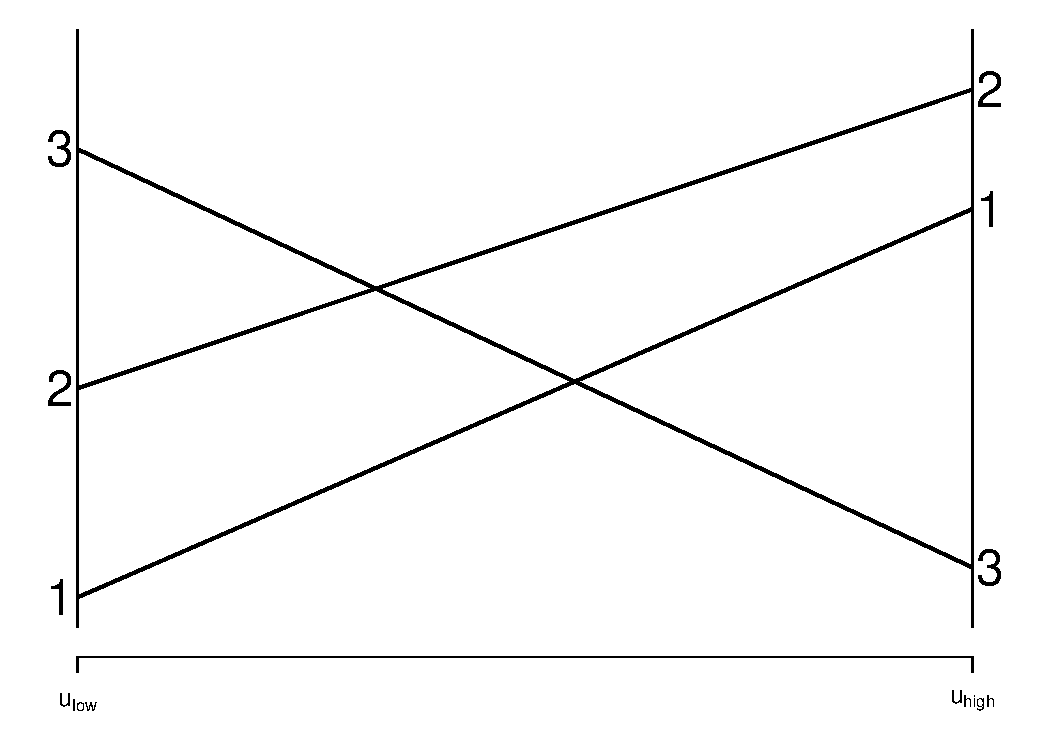
\includegraphics[width=0.5\textwidth]{illustration_inversions.pdf}%
\caption{Three lines in dual space, restricted to the interval $(\ul,\uh]$. If two lines intersect in this interval, the ordering of their values of the $v$-coordinate at $\ul$ and $\uh$ must have turned around. Therefore, the number of IAs in the interval $(\ul,\uh]$ is given by the number of inversions in the permutation $(3 \; 1 \; 2)$.}%
\label{fig:illustrateInversions}%
\end{figure}

For the Theil-Sen estimator, we obtain $n(n-1)$ IAs in dual space, where parallel lines meet at $+\infty$ by convention. Suppose we want to find the $k$-th smallest IA (e.g., $k$ could be $\lfloor (n(n-1)+1)/2\rfloor$ for the lower median). The idea is to maintain a half-open interval $(\ul,\uh]$, which is initialized at $(-\infty, \infty]$ and always contains the IA we are looking for. We also keep a count $L$ and $C$ of the total number of IAs to the left and within the interval respectively. If the number of IAs in the interval is of order $\mathcal{O}(n)$, we can enumerate them  in $\mathcal{O}(n\log(n))$ time and select the desired element (we call this ``brute-force computation''). If there are more IAs left in the interval, we use a contraction strategy which makes the interval $(\ul,\uh]$ progressively smaller while still containing the target $k$-th smallest slope, until it is small enough for brute-force computation.

In order to contract the interval, we randomly sample a $\mathcal{O}(n)$ number of IAs. These are then used to estimate a new interval $(\ul',\uh']\subset (\ul,\uh]$ which contains the target IA with high probability. To check whether the contracted interval contains the target, we count the number of IAs in the intervals $(\ul, \ul']$ and $(\ul',\uh']$. If the current count $L$ added to the number of IAs in the former interval exceeds $k$, we know that the target IA is in $(\ul, \ul']$. If not, we check whether additionally adding the number of IAs in $(\ul',\uh']$ gives a total count exceeding $k$, in which case the target IA is in $(\ul', \uh']$. If neither of those cases hold, we know the target IA is in $(\uh', \uh]$. After the contraction, we update $L$ and $C$ and this process is repeated until $C$, the number of IAs in the current interval, is of the order $\mathcal{O}(n)$. To execute this strategy, we need a method to randomly sample IAs. It turns out that this can be achieved in $\mathcal{O}(n\log(n))$ time, again using an adaptation of merge sort. For the Theil-Sen estimator there is an expected $\mathcal{O}(1)$ number of iterations required for convergence, leading to a total expected complexity of $\mathcal{O}(n\log(n))$.\par
For the repeated median estimator, the algorithm is similar to the previously described algorithm in that it also works with an interval-contraction strategy.
In contrast with the previous algorithm however, we now keep track of the lines for which the median IA falls within the interval, in addition to the number of abscissas on the left and within the current interval for each individual line. In each contraction step, we first sample a $\mathcal{O}(\sqrt{n})$ number of lines for which we know that their median IA lies within the current interval. For each of these lines, a $\mathcal{O}(\sqrt{n})$ number of IAs are now sampled which allow for the estimation of a new interval $(\ul',\uh']\subset (\ul,\uh]$ containing the target slope with high probability. The interval $(\ul,\uh]$ can then be contracted by counting the number of IAs for each line on the left and within $(\ul',\uh']$. As before, the algorithm switches to brute-force computation once the number of IAs in $(\ul,\uh]$ is of the order $\mathcal{O}(n)$.  For this algorithm, there is an expected $\mathcal{O}(\log(n))$ number of contraction steps required, resulting in a total complexity of  $\mathcal{O}(n\log^2(n))$.



The original algorithms were only described for the case where the $x_i$ values are all distinct. In case of duplicate values however, some of the slopes are not defined and the natural way of handling this is by ignoring the undefined slopes and computing the median (or any other order statistic) on the remaining slopes. Fortunately, we can incorporate this into our algorithms by realizing that these duplicate $x_i$ values correspond with parallel lines in dual space. Using the convention that parallel lines in dual space meet at $+\infty$, the (repeated) median slope can be found by appropriately adjusting the value of the order statistic of the slope we want to find. For the Theil-Sen estimator, this means we need to find the order statistic corresponding with $\frac{n(n-1)}{2}-\sum_{i=1}^n{\frac{d_i-1}{2}}$ values, where $d_i$ denotes the number of times the value $x_i$ occurs in the predictor variable. For the repeated median estimator, we only have to adjust the inner median, but the adjustment is dependent on the individual line $i$. More specifically, the order statistic for the inner median needs to be computed on $n-d_i$ values. Note that we can count the number of duplicates easily in $\mathcal{O}(n)$ time and so the overall complexity of the algorithm is not affected by this change. There is one additional complication, namely that of duplicate pairs $(x_i, y_i)$. If such pairs are present, one should be careful with computing the permutation of intersections in dual space given an interval $(\ul, \uh]$. Obtaining such a permutation involves sorting (and ranking) a vector of IAs. However, in case of duplicate pairs, this sorting needs to be done using stable sort. If not, duplicate pairs may randomly produce inversions, yielding sampled IAs at $\infty$ even if the current interval has $\uh < \infty$. In the original algorithm, this scenario was not considered and thus not explicitly accounted for. These changes have been incorporated in the implementation provided in the \pkg{robslopes} package.


\section{Implementation and usage}\label{sec:impl}
We briefly describe the implementation and usage of the functions in the \pkg{robslopes} package. The package revolves around 2 main functions, the \code{TheilSen} function and the \code{RepeatedMedian} function, both returning a list with the self-explanatory elements \code{intercept} and \code{slope}. 
 Both functions start with input checking and duplicate counting, which are done in R. The duplicate counts are then used to set the correct target order statistics for the main part of the algorithm. This information is then passed on to the randomized algorithms which are implemented in C++, making use of the \CRANpkg{rcpparmadillo} package \citep{eddelbuettel2011rcpp, rcpparmadillo}. \par

The \code{TheilSen} function has the layout \code{TheilSen(x, y, alpha = NULL, verbose = TRUE)}, where the \code{x} and \code{y} arguments are the input vectors for the predictor and response variable respectively. The \code{verbose} option allows for switching off the printing of the computation progress.
Finally, the \code{alpha} argument is a value between 0 and 1 which determines the order statistic corresponding with the target slope. When \code{alpha = NULL}, the default, the upper median  of the $m$ slopes is computed, which corresponds with the $\lfloor (m + 2) / 2\rfloor$-th order statistic. For any other value of $0\leq$\code{alpha}$\leq 1$, the function computes the $[$\code{alpha}$\;m]$-th order statistic of the slopes, where $[\cdot]$ is the rounding operator.\par

The \code{RepeatedMedian} function has the layout \code{RepeatedMedian(x, y, alpha = NULL, beta = NULL, verbose = TRUE)}, where the \code{x}, \code{y} and \code{verbose} arguments play the same role as for the \code{TheilSen} function. The arguments \code{alpha} and \code{beta} determine the order statistics of the inner and outer ``median''. When \code{NULL}, the default, they again correspond to the upper median. If they contain values between zero and one, the order statistics corresponding with the inner and outer ``median'' are given by $[$\code{alpha}$\;m]$ and $[$\code{beta}$\;m]$ respectively.\par

For convenience, the \code{TheilSen} and \code{RepeatedMedian} functions have been wrapped in the user-friendly functions \code{robslope} and \code{robslope.fit}. These mimic the structure of common regression functions (e.g., \code{lm} and \code{lm.fit}). In particular, \code{robslope} takes the standard arguments \code{formula}, \code{data}, \code{subset}, \code{weights} and \code{na.action}, in addition to the \code{type} argument selecting which type of slope to compute, as well as the optional \code{alpha}, \code{beta} and \code{verbose} arguments of the \code{TheilSen} and \code{RepeatedMedian} functions.\par 

As an example we analyze the flights data of the \CRANpkg{nycflights13} package \citep{R:nycflights}. It contains on-time data for all flights that departed in New York City (i.e. JFK, LGA or EWR airports) in 2013. We consider the distance traveled in miles as the predictor variable, and take the air time in minutes as the response. After removing all NA values, we end up with a data set of 327,346 observations. In contrast to the previous example, this one is too large to compute the TS or RM slope with a brute-force algorithm (on most computers). We now calculate the TS and RM slopes three times each, where we change the inner order statistic to the first, second and third quartiles. With the exception of graphical parameters, the code executed is shown below.

\begin{example}
library("robslopes")
library("nycflights13")
data("flights")

ts.out.25 <- robslope(formula = air_time~distance, data = data, alpha = 0.25)
ts.out.50 <- robslope(formula = air_time~distance, data = data, alpha = 0.50)
ts.out.75 <- robslope(formula = air_time~distance, data = data, alpha = 0.75)
plot(data$distance, data$air_time)
abline(coef(ts.out.25), col = "red", lwd = 3)
abline(coef(ts.out.50), col = "green", lwd = 3)
abline(coef(ts.out.75), col = "blue", lwd = 3)

rm.out.25 <- robslope(formula = air_time~distance, data = data, beta = 0.25,
                      type = "RepeatedMedian")
rm.out.50 <- robslope(formula = air_time~distance, data = data, beta = 0.50,
                      type = "RepeatedMedian")
rm.out.75 <- robslope(formula = air_time~distance, data = data, beta = 0.75,
                      type = "RepeatedMedian")
plot(data$distance, data$air_time)
abline(coef(rm.out.25), col = "red", lwd = 3)
abline(coef(rm.out.50), col = "green", lwd = 3)
abline(coef(rm.out.75), col = "blue", lwd = 3)

\end{example}
%\begin{example}
%library("nycflights13")
%data("flights")
%x <- data$distance
%y <- data$air_time
%
%ts.out.25 <- robslopes::robslope(formula = air_time~distance, data = data, alpha = 0.25)
%ts.out.25 <- robslopes::TheilSen(x, y, beta = 0.25, verbose = FALSE)
%ts.out.50 <- robslopes::TheilSen(x, y, beta = 0.50, verbose = FALSE)
%ts.out.75 <- robslopes::TheilSen(x, y, beta = 0.75, verbose = FALSE)
%plot(x, y)
%abline(ts.out.25$intercept, ts.out.25$slope, col = "red", lwd = 3)
%abline(ts.out.50$intercept, ts.out.50$slope, col = "green", lwd = 3)
%abline(ts.out.75$intercept, ts.out.75$slope, col = "blue", lwd = 3)
%
%rm.out.25 <- robslopes::RepeatedMedian(x, y, beta = 0.25, verbose = FALSE)
%rm.out.50 <- robslopes::RepeatedMedian(x, y, beta = 0.50, verbose = FALSE)
%rm.out.75 <- robslopes::RepeatedMedian(x, y, beta = 0.75, verbose = FALSE)
%plot(x, y)
%abline(rm.out.25$intercept, rm.out.25$slope, col = "red", lwd = 3)
%abline(rm.out.50$intercept, rm.out.50$slope, col = "green", lwd = 3)
%abline(rm.out.75$intercept, rm.out.75$slope, col = "blue", lwd = 3)
%\end{example}

The resulting figure is shown in Figure \ref{fig:flights}. In this example, the slopes calculated by the TS and RM estimators are virtually identical due to the very limited number of outliers and the large number of data points. Note that there are many duplicates in this data set, which are handled appropriately by the proposed implementation. 

\begin{figure}[!ht]%
\centering
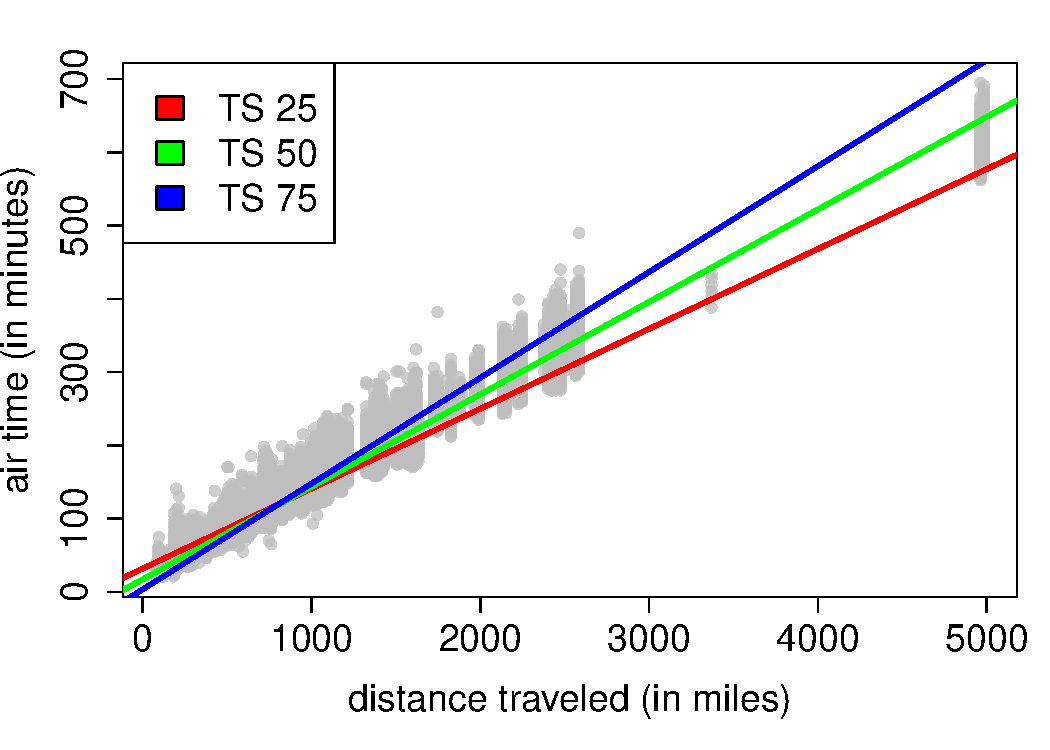
\includegraphics[width=0.48\textwidth]{flights_example_TS}
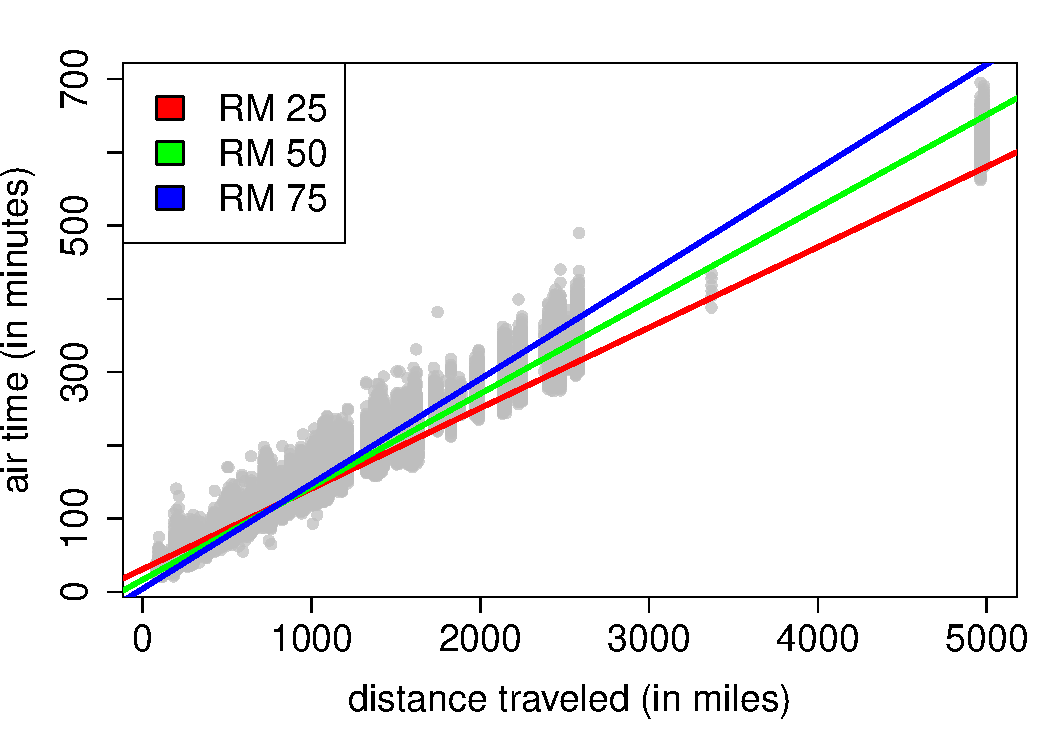
\includegraphics[width=0.48\textwidth]{flights_example_RM}%
\caption{The TS (left) and RM (right) slopes fitted on the flights data. The first, second and third quartiles as the (inner) order statistic are shown in red, green and blue respectively. The slopes are virtually identical for both estimators in this example, as there are not many outliers in the data. The implemented algorithm appropriately deals with the many duplicate $x$-values in this data set.}%
\label{fig:flights}%
\end{figure}

\section{Benchmarking study}\label{sec:bench}

We now benchmark the implemented algorithm against the existing implementations in the \pkg{deming}, \pkg{zyp}, \pkg{mblm}, and \pkg{RobustLinearReg} packages. Note that the \pkg{deming} and \pkg{zyp} packages only contain the TS estimator, the others contain both the TS and RM estimators. All simulations were done using the R-package \CRANpkg{microbenchmark} \citep{microbenchmark} and were run  on an Intel\textsuperscript{\textregistered} Core\textsuperscript{\texttrademark} i7-10750H @2.60GHz processor. The setup is as follows. For each value of $n = \{10, 10^2, 10^3, 10^4\}$, we have generated 100 samples $(x_i,y_i)$ from the bivariate standard normal distribution. Afterward, each of the available implementations was used to estimate the regression parameters and the execution time was measured (in nanoseconds).\par

The following code snippets show the code used for benchmarking the TS and RM estimator for a sample of size $n = 10^3$, the same code was used for the other sample sizes, with exception of $n = 10^4$, in which case the implementation of the \pkg{mblm} package was left out due to its computational burden (it takes several hours to compute it once).

\begin{example}
n   <- 10^3
mbm <- microbenchmark("deming" = deming::theilsen(y~x, data = data),
                      "zyp" = zyp::zyp.sen(y~x, dataframe = data),
                      "mblm" = mblm::mblm(y~x, dataframe = data, repeated = FALSE),
                      "RobustLinearReg" = RobustLinearReg::theil_sen_regression(y~x,
		      data = data),
                      "robslopes" = robslopes::TheilSen(x, y),
                      setup = {x = rnorm(n); y = rnorm(n);
                      data = as.data.frame(cbind(x, y))}, times = 100)
autoplot(mbm)
\end{example}


\begin{example}
n   <- 10^3
mbm <- microbenchmark("mblm" = mblm::mblm(y~x, dataframe = data, repeated = TRUE),
                      "RobustLinearReg" = RobustLinearReg::siegel_regression(y~x,
		      data = data),
                      "robslopes" = robslopes::RepeatedMedian(x, y),
                      setup = {x = rnorm(n); y = rnorm(n);
                      data = as.data.frame(cbind(x, y))}, times = 100)
autoplot(mbm)
\end{example}
										

Figure \ref{fig:bench_TS} shows the results for the Theil-Sen estimator. We see that for the smallest sample size, $n = 10$, the absolute computation times are extremely low and while there are visible differences, they are probably not of practical relevance. For $n=100$, the \pkg{robslopes} package is roughly five times faster than the fastest competitor, and the \pkg{mblm} implementation starts to run away from the other competitors.  For $n = 10^3$, the differences become much clearer. The \pkg{robslopes} implementation is now between one and two orders of magnitude faster than the best competitor. Finally, for $n = 10^4$ the gap widens further to a difference of over two orders of magnitude. Note that for $n = 10^4$, we have left out the \pkg{mblm} package in the comparison as a single run takes several hours and the resulting plot would hinder a clear comparison.

\begin{figure}[h]
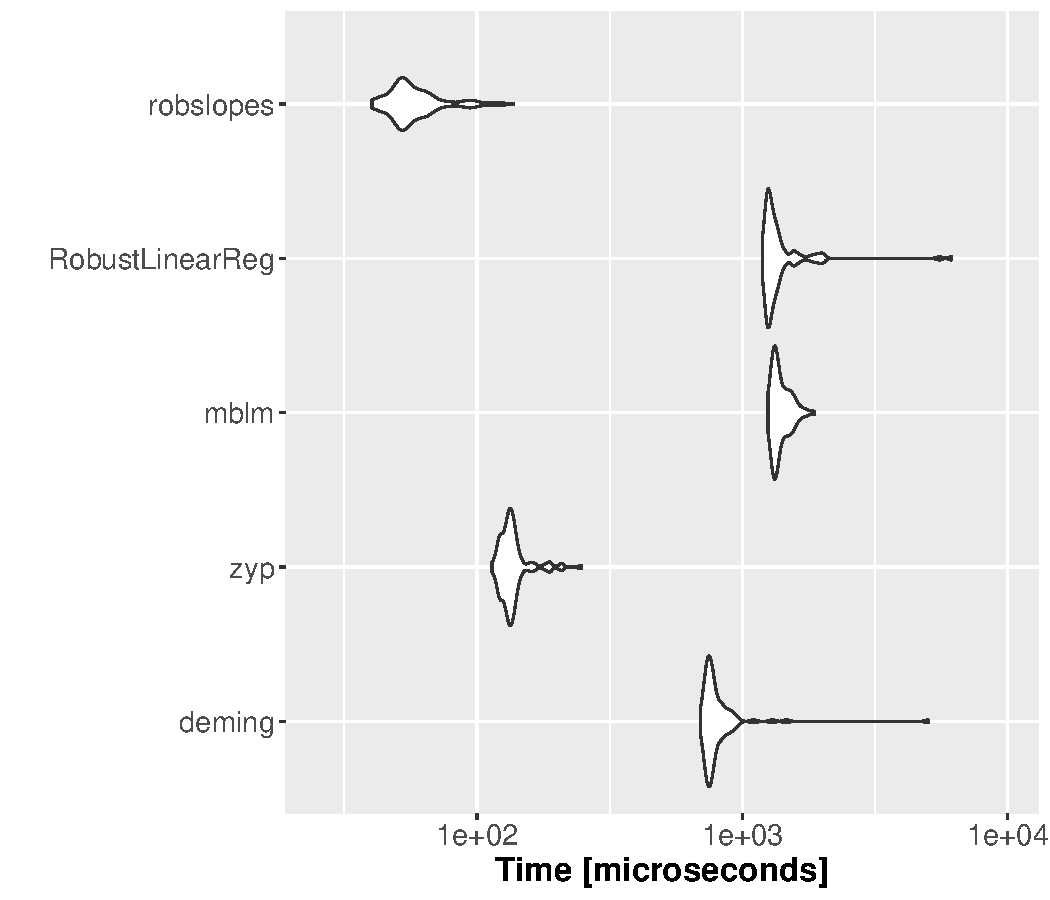
\includegraphics[width = 0.45\textwidth]{benchmark_TS_10.pdf}
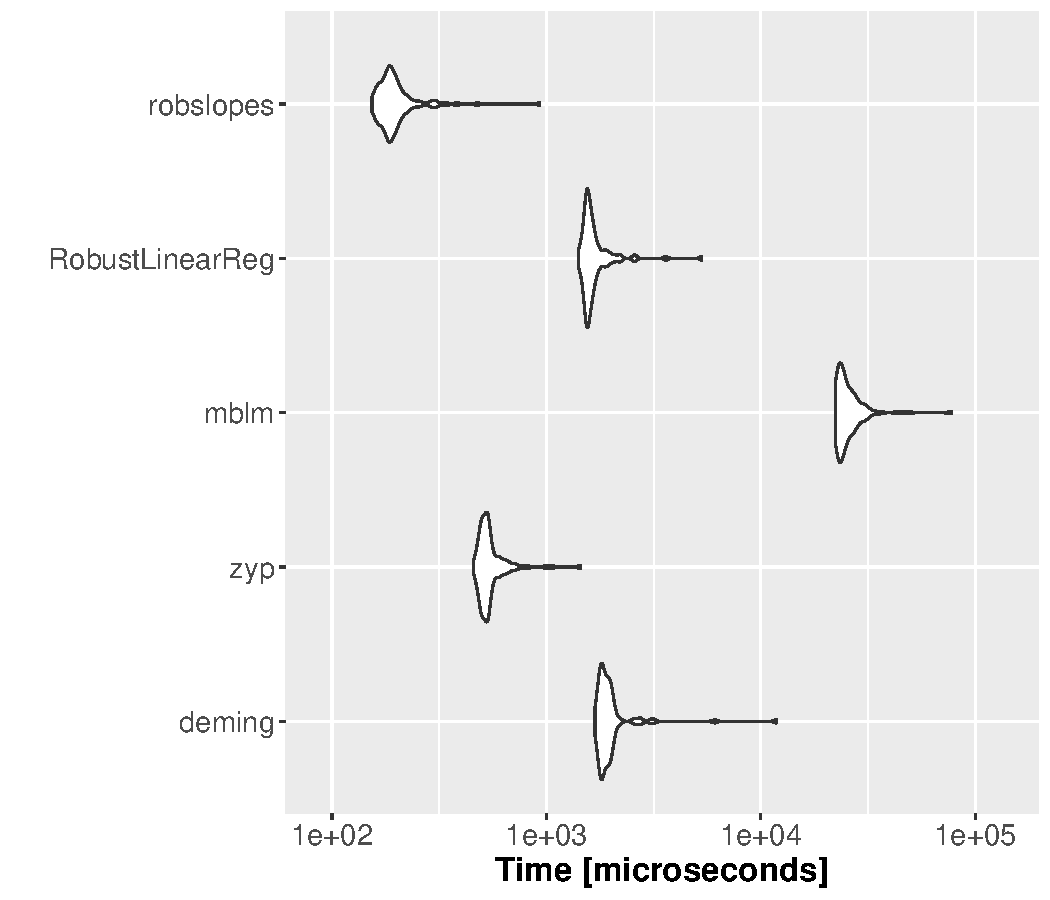
\includegraphics[width = 0.45\textwidth]{benchmark_TS_100.pdf}
\vfill
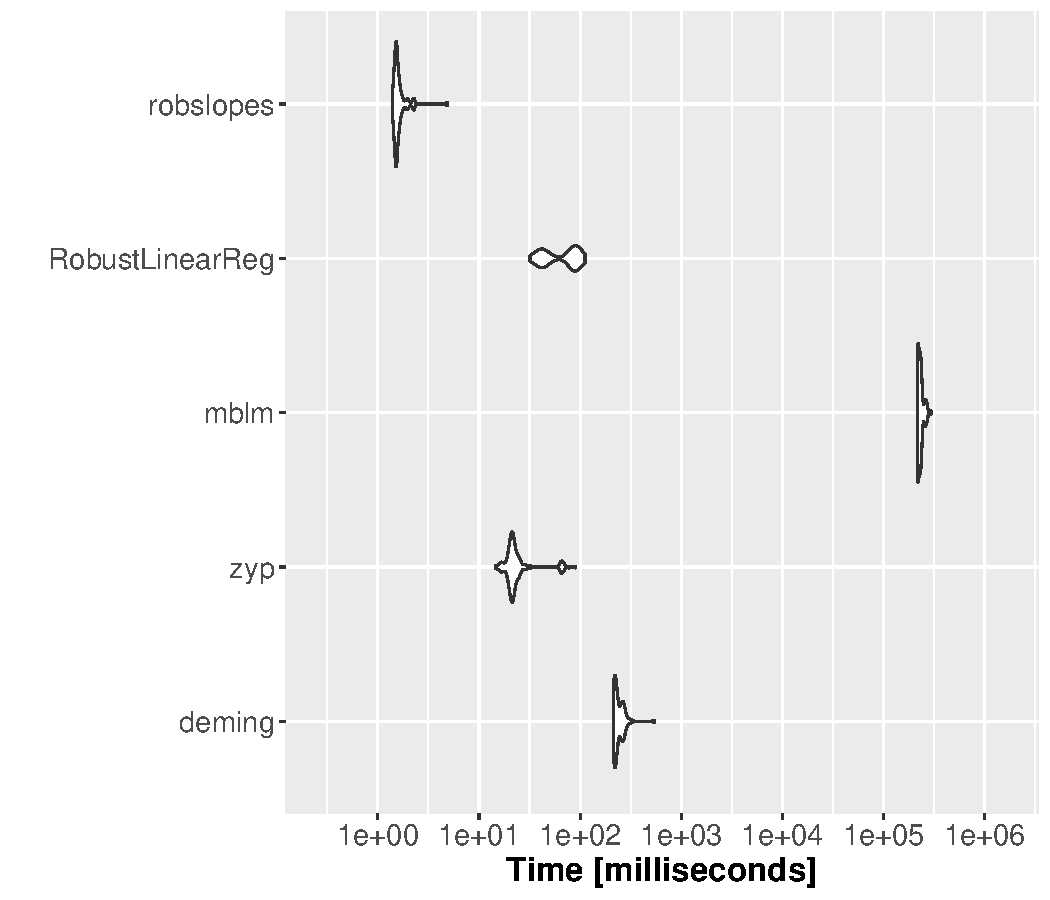
\includegraphics[width = 0.45\textwidth]{benchmark_TS_1000.pdf}
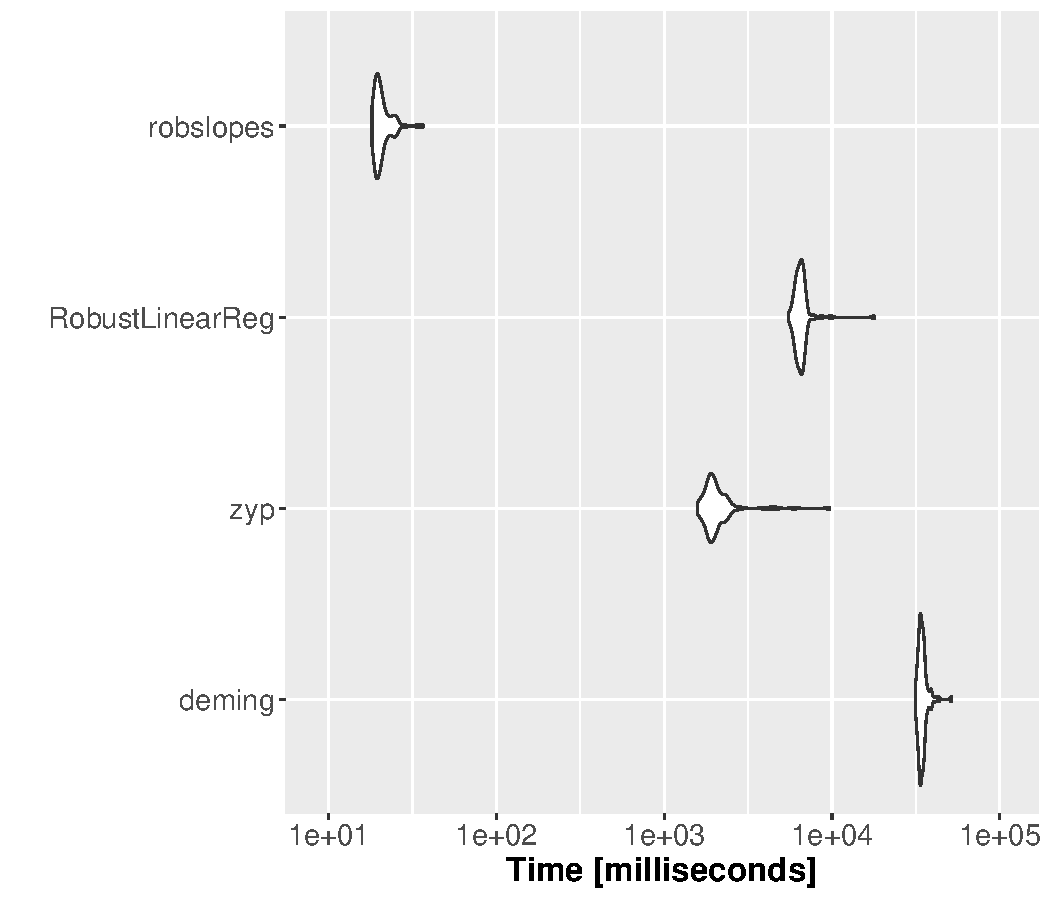
\includegraphics[width = 0.45\textwidth]{benchmark_TS_10000.pdf}
\caption{Computation times of the different implementations of the Theil-Sen slope estimator for the sample size $n$ equal to $10$, $10^2$, $10^3$ and $10^4$ in the top left, top right, bottom left and bottom right panels respectively. The \pkg{robslopes} implementation is consistently faster than the competition by orders of magnitude. The difference scales close to linearly in $n$, gaining almost one order of magnitude advantage for a similar increase in the sample size, which is what we expect based on the theoretical computational complexities. The \pkg{mblm} estimator was left out for sample size $n=10^4$ due to it requiring several hours to compute once.}
\label{fig:bench_TS}
\end{figure}



Figure \ref{fig:bench_RM} shows the results for the RM estimator. As for the TS estimator, the difference in computation time is already visible for small sample sizes of $n=10$ and $n=100$, where the \pkg{robslopes} implementation is roughly a factor 20 faster than the competition. However, the absolute computation times for these sample sizes is by no means prohibitive for any of the implementations. Starting at $n = 1000$ however, we start to see a larger difference, especially between the \pkg{robslopes} and \pkg{mblm} implementations. The former is now roughly 800 times faster than the latter, and 60 times faster than the \pkg{RobustLinearReg} implementation. For sample size $n = 10^4$, we did not include the \pkg{mblm} implementation as it now takes roughly half an hour to compute, in contrast with 16 seconds for the \pkg{RobustLinearReg} implementation and 0.034 seconds (on average) for the \pkg{robslopes} implementation. Finally note that interestingly, the repeated median of the \pkg{mblm} package is much faster than the Theil-Sen estimator of the same package. This is somewhat counter-intuitive, but turns out to be caused by a much higher number of calls to the \code{c()} function (concatenate) in the implementation of the TS estimator.

\begin{figure}[h]
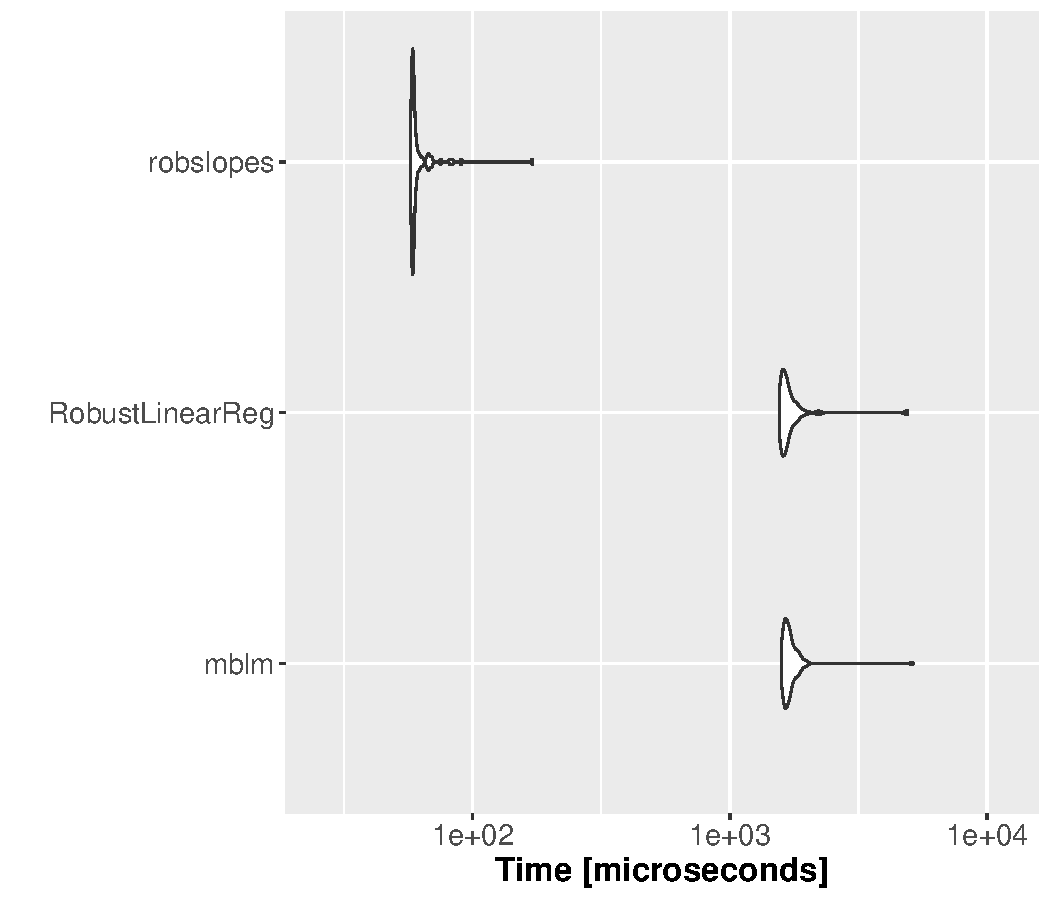
\includegraphics[width = 0.45\textwidth]{benchmark_RM_10.pdf}
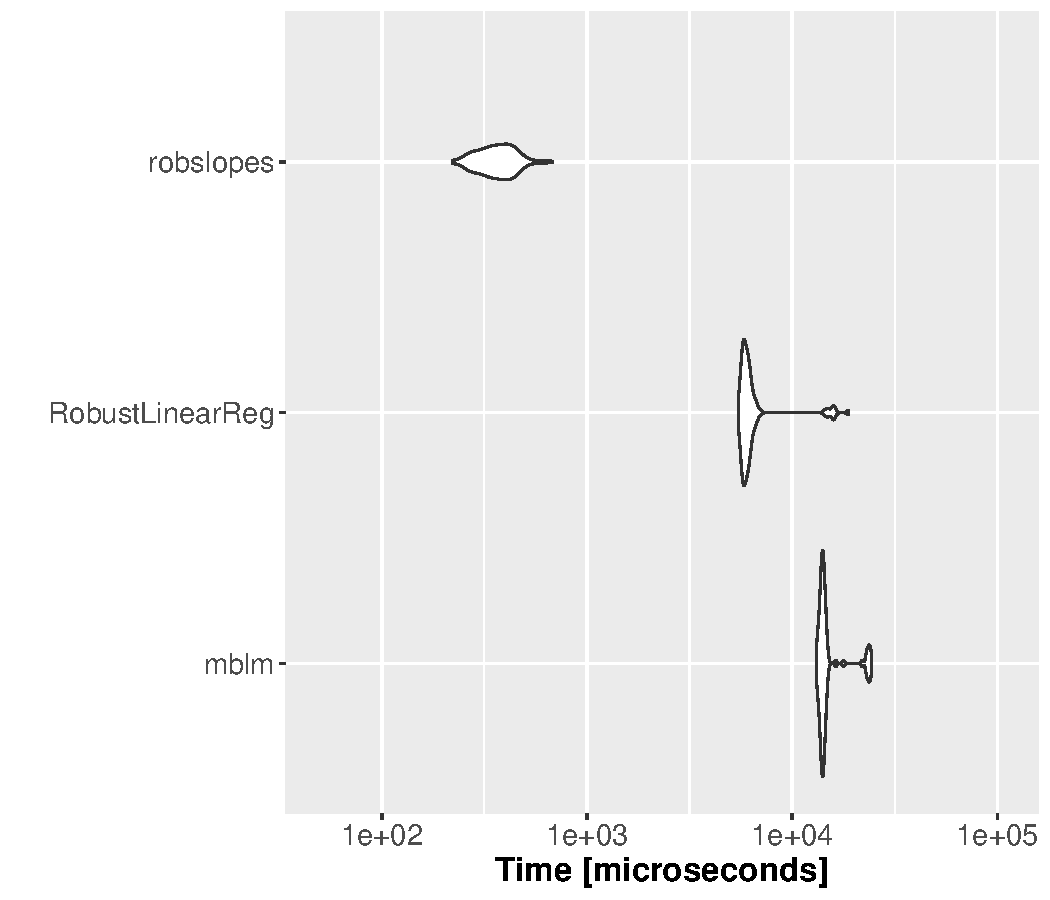
\includegraphics[width = 0.45\textwidth]{benchmark_RM_100.pdf}
\vfill
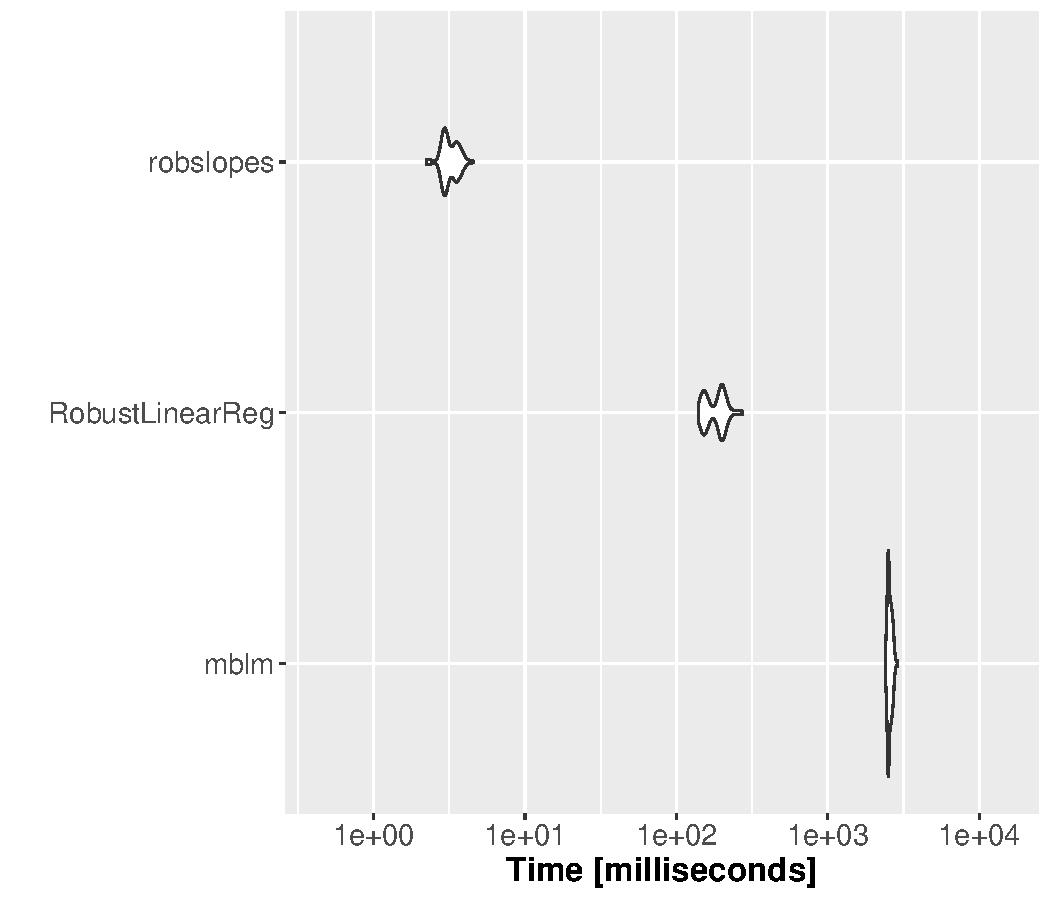
\includegraphics[width = 0.45\textwidth]{benchmark_RM_1000.pdf}
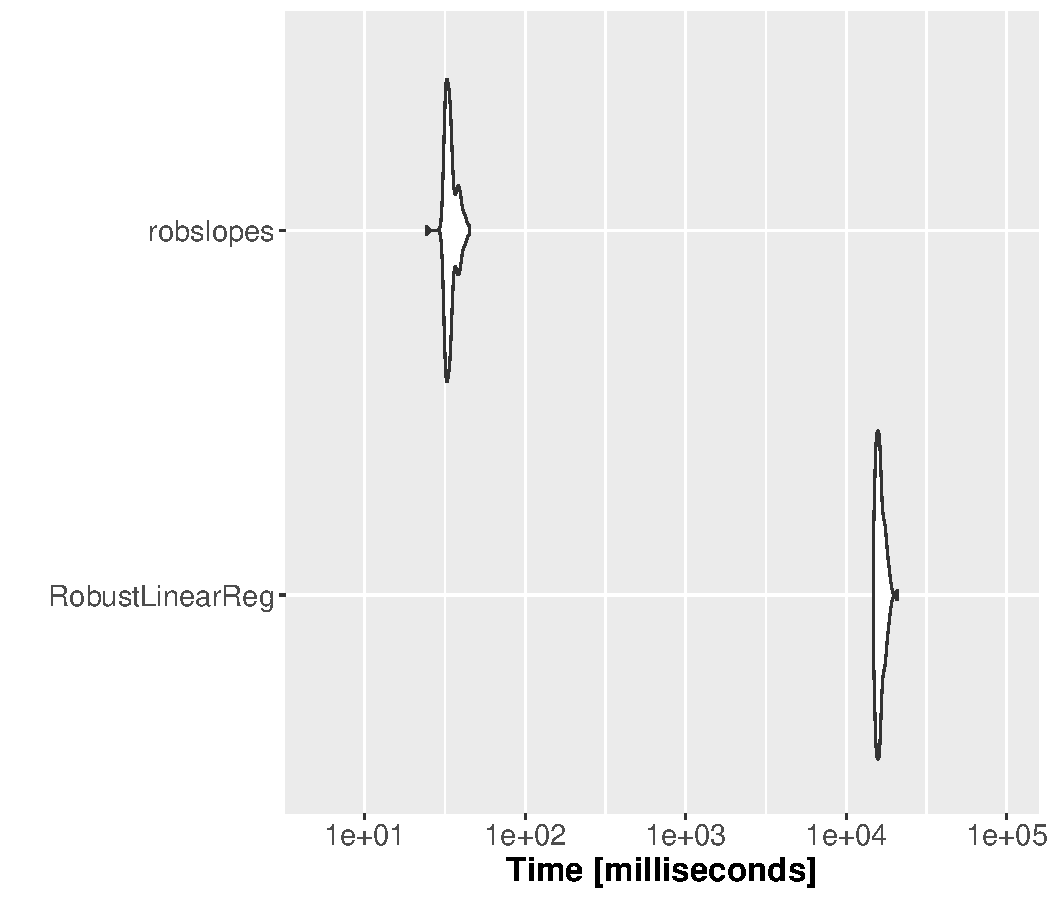
\includegraphics[width = 0.45\textwidth]{benchmark_RM_10000.pdf}
\caption{Computation times of the different implementations of the repeated median slope estimator for the sample size $n$ equal to $10$, $10^2$, $10^3$ and $10^4$ in the top left, top right, bottom left and bottom right panels respectively. The \pkg{robslopes} implementation is consistently faster than the competition by orders of magnitude. The difference scales close to linearly in $n$, which is what we expect based on the theoretical computational complexities.
Note that the \pkg{mblm} estimator was left out for sample size $n=10^4$ due to it requiring more than $10^6$ milliseconds (approx. 30 minutes) to compute.}
\label{fig:bench_RM}
\end{figure}

As explained before, the brute-force implementations of the (repeated) median slope require $\mathcal{O}(n^2)$ storage as they typically compute all slopes and store them in a $n\times n$ matrix. Therefore, while a sample size of $n=10^4$ is by no means extremely large, we cannot go much higher than that. A sample size of $n=10^5$ for example, would require a RAM memory of about 75GB, which is rather uncommon on most computers and laptops. The implementations in the \pkg{robslopes} package however, require only $\mathcal{O}(n)$ storage space, and we can thus easily compute the estimators on much larger samples. To illustrate this, we have continued the benchmarking study with only the \pkg{robslopes} implementation, but this time for the sample sizes $n = 10^5, 10^6$ and $10^7$. This was done using the following code snippet, where the saving of the results in the for loop is omitted:

\begin{example}
for (n in 10^(5:7)) {
	mbm <- microbenchmark("robslopes" = robslopes::TheilSen(x, y),
                     setup = {x = rnorm(n); y = rnorm(n);
                     data = as.data.frame(cbind(x, y))}, times = 100)
}	

for (n in 10^(5:7)) {
	mbm <- microbenchmark("robslopes" = robslopes::RepeatedMedian(x, y),
                     setup = {x = rnorm(n); y = rnorm(n);
                     data = as.data.frame(cbind(x, y))}, times = 100)
}												
\end{example}

Figure \ref{fig:bench_largen} shows the mean computation times of the TS estimator and the RM estimator for sample sizes up to $n = 10^7$. As an example, for a sample size of $n=10^6$, the TS estimator requires roughly 4 seconds of computation time, whereas the RM estimator requires roughly 6 seconds. The blue shade on the figure indicates the maximum and minimum computation time over the 100 replications, showing that the computation times have a fairly small variance around their mean. The red line shows a (robustly) estimated fit of the theoretical computation times to the observed ones (i.e. of the functions $f(n) = \beta n \log(n)$ and $f(n) = \beta n \log^2(n)$ for a $\beta \in \mathbb{R}$), indicating that for $n\geq 10^3$, the observed computational cost grows according to the theoretical complexity.

\begin{figure}[h]
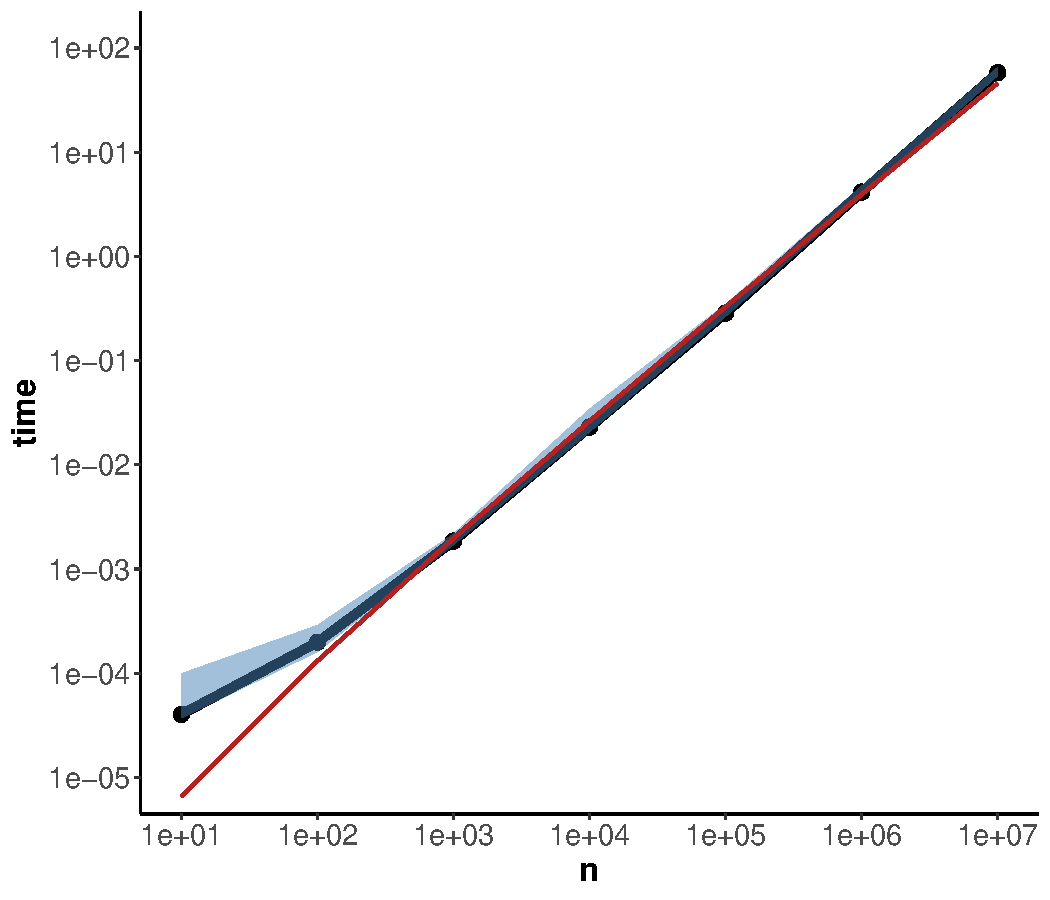
\includegraphics[width = 0.45\textwidth]{benchmark_largen_TS.pdf}
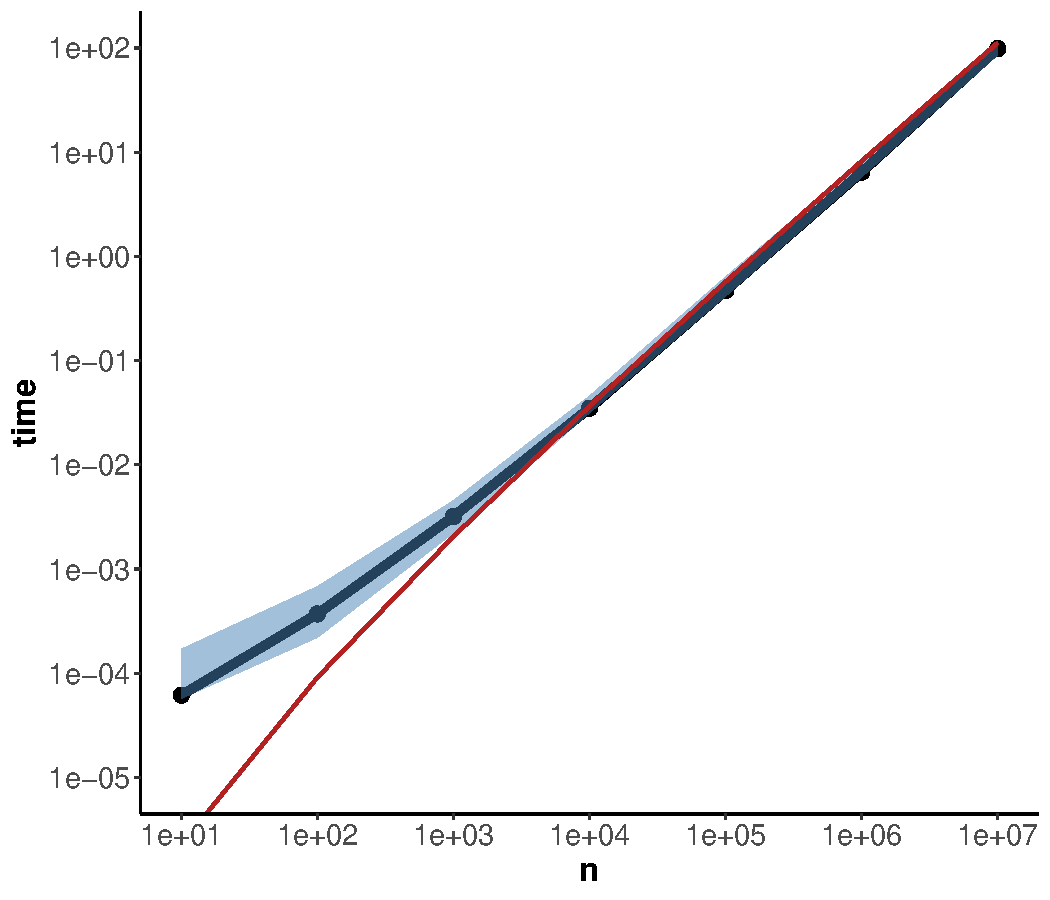
\includegraphics[width = 0.45\textwidth]{benchmark_largen_RM.pdf}
\caption{Mean computation times of the Theil-Sen (left) and repeated median (right) estimators as implemented in \pkg{robslopes} for increasing sample size $n$. The red line is an estimate of the $\sim n\log(n)$ (for TS) and $\sim n\log^2(n)$ (for RM) expected computational cost. The blue shade indicates the minimum and maximum computation times. Other than the deviations for very small $n$ which are due to computational overhead, the computational cost scales precisely as the theory predicts. Furthermore, the variance of the computation times around their mean is negligible.}
\label{fig:bench_largen}
\end{figure}

\clearpage
\section{Summary}\label{sec:conc}
We have introduced the \pkg{robslopes} package which contains fast implementations of the popular Theil-Sen and repeated
median slope estimators. The implemented algorithms are randomized algorithms running in quasilinear expected time and use linear space. In contrast, the currently available implementations in different R packages on CRAN require quadratic time and space. A benchmark study comparing the common implementations of the slope estimator with the newly introduced one illustrates speedups up to a factor $10^3$ compared with the next best alternative implementation for common sample sizes. Additionally, due to the linear space requirements of the algorithms, the slope estimators can be computed on much larger sample sizes than the current maximum. Finally, the original algorithms were adjusted to properly deal with potential duplicates in the predictor variable.\par
The fast implementation of these popular slope estimators unlocks new possibilities for their use in modern applications where the slope has to be estimated repeatedly and on a large number of data points. Evidently, inferential procedures based on bootstrapping are also highly facilitated by these fast algorithms. Finally, the underlying C++ implementation may serve as a useful reference for implementations of these algorithms in other programming languages, which also seem to be scarce.

\bibliography{raymaekers}

		

\address{Jakob Raymaekers\\
  Maastricht University and KU Leuven \\
  Maastricht University, Department of Quantitative Economics\\
 6200 MD Maastricht\\
  The Netherlands\\
  \email{j.raymaekers@maastrichtuniversity.nl}\\
  also \\
KU Leuven, Department of Mathematics\\
 3001 Leuven\\
  Belgium\\
  \email{jakob.raymaekers@kuleuven.be}}
		
